\documentclass{article}
\usepackage[latin1]{inputenc}
\usepackage{amsmath}
\usepackage{amsfonts}
\usepackage{amssymb}
\usepackage{graphicx}
\usepackage{tikz}
\usepackage[margin=1in]{geometry}
\title{Bridge Project Cleaning Documentation}
\begin{document}
\maketitle
\begin{center}


\tikzset{every picture/.style={line width=0.75pt}} %set default line width to 0.75pt        

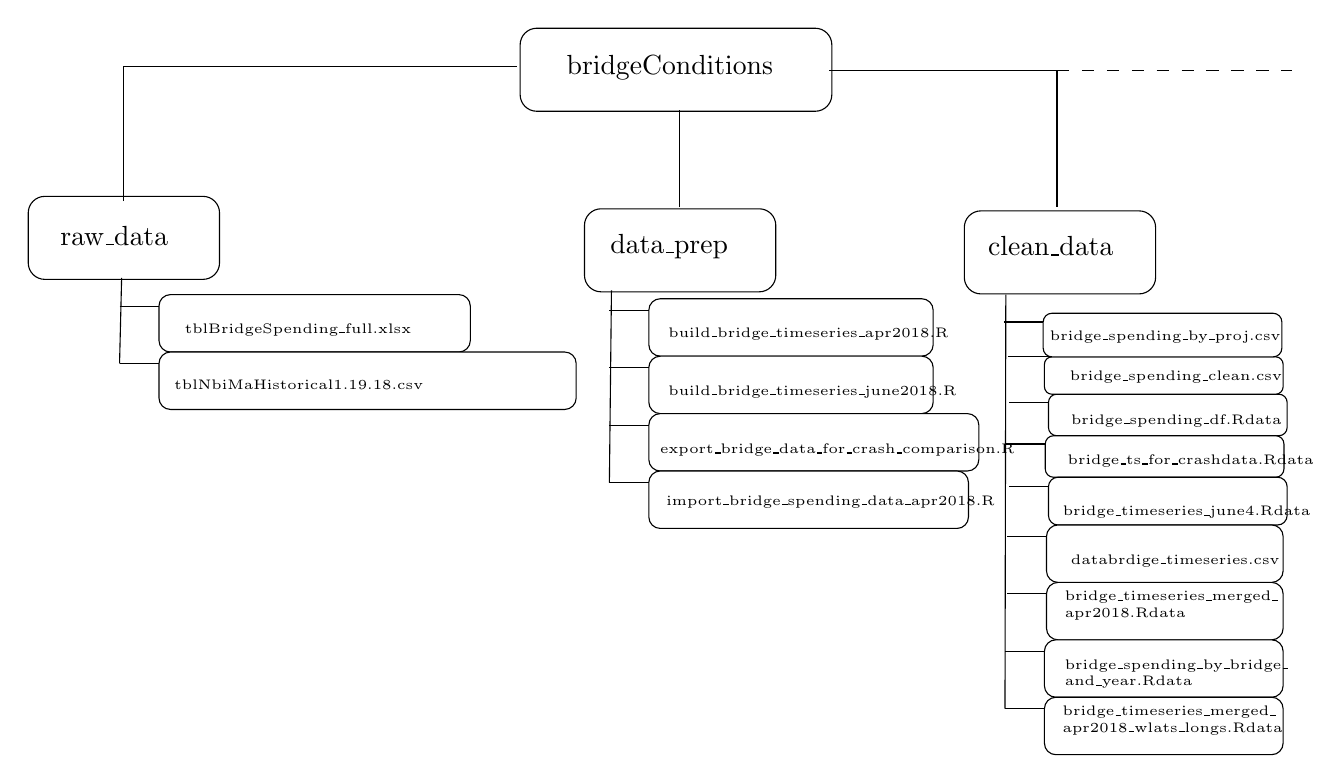
\begin{tikzpicture}[x=0.75pt,y=0.75pt,yscale=-1,xscale=1]
%uncomment if require: \path (0,413); %set diagram left start at 0, and has height of 413

%Rounded Rect [id:dp3299205573966941] 
\draw  [fill={rgb, 255:red, 255; green, 255; blue, 255 }  ,fill opacity=1 ] (253.83,44) .. controls (253.83,39.58) and (257.42,36) .. (261.83,36) -- (396,36) .. controls (400.42,36) and (404,39.58) .. (404,44) -- (404,68) .. controls (404,72.42) and (400.42,76) .. (396,76) -- (261.83,76) .. controls (257.42,76) and (253.83,72.42) .. (253.83,68) -- cycle ;
%Rounded Rect [id:dp4953706636868318] 
\draw  [fill={rgb, 255:red, 255; green, 255; blue, 255 }  ,fill opacity=1 ] (16.83,125) .. controls (16.83,120.58) and (20.42,117) .. (24.83,117) -- (101,117) .. controls (105.42,117) and (109,120.58) .. (109,125) -- (109,149) .. controls (109,153.42) and (105.42,157) .. (101,157) -- (24.83,157) .. controls (20.42,157) and (16.83,153.42) .. (16.83,149) -- cycle ;
%Rounded Rect [id:dp3869379102082733] 
\draw  [fill={rgb, 255:red, 255; green, 255; blue, 255 }  ,fill opacity=1 ] (284.83,131) .. controls (284.83,126.58) and (288.42,123) .. (292.83,123) -- (369,123) .. controls (373.42,123) and (377,126.58) .. (377,131) -- (377,155) .. controls (377,159.42) and (373.42,163) .. (369,163) -- (292.83,163) .. controls (288.42,163) and (284.83,159.42) .. (284.83,155) -- cycle ;
%Rounded Rect [id:dp9021191134275666] 
\draw  [fill={rgb, 255:red, 255; green, 255; blue, 255 }  ,fill opacity=1 ] (467.83,132) .. controls (467.83,127.58) and (471.42,124) .. (475.83,124) -- (552,124) .. controls (556.42,124) and (560,127.58) .. (560,132) -- (560,156) .. controls (560,160.42) and (556.42,164) .. (552,164) -- (475.83,164) .. controls (471.42,164) and (467.83,160.42) .. (467.83,156) -- cycle ;
%Straight Lines [id:da486167121400217] 
\draw    (62.83,119.33) -- (62.83,54.33) ;
%Straight Lines [id:da9474608679677452] 
\draw    (62.83,54.33) -- (252.5,54.33) ;
%Straight Lines [id:da5933582120104823] 
\draw    (330.5,122.33) -- (330.5,75.33) ;
%Rounded Rect [id:dp9301611879825988] 
\draw  [fill={rgb, 255:red, 255; green, 255; blue, 255 }  ,fill opacity=1 ] (79.83,169.87) .. controls (79.83,166.81) and (82.31,164.33) .. (85.37,164.33) -- (224.3,164.33) .. controls (227.36,164.33) and (229.83,166.81) .. (229.83,169.87) -- (229.83,186.47) .. controls (229.83,189.52) and (227.36,192) .. (224.3,192) -- (85.37,192) .. controls (82.31,192) and (79.83,189.52) .. (79.83,186.47) -- cycle ;
%Straight Lines [id:da7323944236282891] 
\draw    (402.83,56.33) -- (512.5,56.33) ;
%Straight Lines [id:da77539301409979] 
\draw    (512.5,56.33) -- (512.5,122.33) ;
%Straight Lines [id:da4830898578227125] 
\draw  [dash pattern={on 4.5pt off 4.5pt}]  (512.5,56.33) -- (625.5,56.33) ;
%Rounded Rect [id:dp5669144322763333] 
\draw  [fill={rgb, 255:red, 255; green, 255; blue, 255 }  ,fill opacity=1 ] (79.83,197.53) .. controls (79.83,194.48) and (82.31,192) .. (85.37,192) -- (275.3,192) .. controls (278.36,192) and (280.83,194.48) .. (280.83,197.53) -- (280.83,214.13) .. controls (280.83,217.19) and (278.36,219.67) .. (275.3,219.67) -- (85.37,219.67) .. controls (82.31,219.67) and (79.83,217.19) .. (79.83,214.13) -- cycle ;
%Rounded Rect [id:dp7084920372414294] 

%Rounded Rect [id:dp33954491738600545] 

%Rounded Rect [id:dp6156154944564061] 
\draw  [fill={rgb, 255:red, 255; green, 255; blue, 255 }  ,fill opacity=1 ] (315.83,171.87) .. controls (315.83,168.81) and (318.31,166.33) .. (321.37,166.33) -- (447.3,166.33) .. controls (450.36,166.33) and (452.83,168.81) .. (452.83,171.87) -- (452.83,188.47) .. controls (452.83,191.52) and (450.36,194) .. (447.3,194) -- (321.37,194) .. controls (318.31,194) and (315.83,191.52) .. (315.83,188.47) -- cycle ;
%Rounded Rect [id:dp9023582623722428] 
\draw  [fill={rgb, 255:red, 255; green, 255; blue, 255 }  ,fill opacity=1 ] (315.83,199.53) .. controls (315.83,196.48) and (318.31,194) .. (321.37,194) -- (447.3,194) .. controls (450.36,194) and (452.83,196.48) .. (452.83,199.53) -- (452.83,216.13) .. controls (452.83,219.19) and (450.36,221.67) .. (447.3,221.67) -- (321.37,221.67) .. controls (318.31,221.67) and (315.83,219.19) .. (315.83,216.13) -- cycle ;
%Rounded Rect [id:dp7948102013304517] 
\draw  [fill={rgb, 255:red, 255; green, 255; blue, 255 }  ,fill opacity=1 ] (315.83,227.2) .. controls (315.83,224.14) and (318.31,221.67) .. (321.37,221.67) -- (469.3,221.67) .. controls (472.36,221.67) and (474.83,224.14) .. (474.83,227.2) -- (474.83,243.8) .. controls (474.83,246.86) and (472.36,249.33) .. (469.3,249.33) -- (321.37,249.33) .. controls (318.31,249.33) and (315.83,246.86) .. (315.83,243.8) -- cycle ;
%Rounded Rect [id:dp9410694337910341] 
\draw  [fill={rgb, 255:red, 255; green, 255; blue, 255 }  ,fill opacity=1 ] (315.83,254.87) .. controls (315.83,251.81) and (318.31,249.33) .. (321.37,249.33) -- (464.3,249.33) .. controls (467.36,249.33) and (469.83,251.81) .. (469.83,254.87) -- (469.83,271.47) .. controls (469.83,274.52) and (467.36,277) .. (464.3,277) -- (321.37,277) .. controls (318.31,277) and (315.83,274.52) .. (315.83,271.47) -- cycle ;
%Straight Lines [id:da30901238103944073] 
\draw    (61.83,156.33) -- (60.83,197.53) ;
%Straight Lines [id:da07003316170157703] 
\draw    (60.83,169.87) -- (79.83,169.87) ;
%Straight Lines [id:da1603456728777688] 
\draw    (60.83,197.53) -- (79.83,197.53) ;
%Straight Lines [id:da6394843348079655] 

%Straight Lines [id:da7981296144875458] 

%Straight Lines [id:da6786750525665359] 
\draw    (297.83,162.33) -- (296.83,254.87) ;
%Straight Lines [id:da18131164913333353] 
\draw    (296.83,254.87) -- (315.83,254.87) ;
%Straight Lines [id:da7262882382271638] 
\draw    (296.83,227.2) -- (315.83,227.2) ;
%Straight Lines [id:da9493301946837864] 
\draw    (296.83,199.53) -- (315.83,199.53) ;
%Straight Lines [id:da33131338226222384] 
\draw    (296.83,171.87) -- (315.83,171.87) ;
%Straight Lines [id:da7640684675283786] 
\draw    (487.83,164.33) -- (487.43,363.87) ;
%Rounded Rect [id:dp21033381099548043] 
\draw  [fill={rgb, 255:red, 255; green, 255; blue, 255 }  ,fill opacity=1 ] (508.37,216.33) .. controls (508.37,214.12) and (510.16,212.33) .. (512.37,212.33) -- (619.37,212.33) .. controls (621.58,212.33) and (623.37,214.12) .. (623.37,216.33) -- (623.37,228.33) .. controls (623.37,230.54) and (621.58,232.33) .. (619.37,232.33) -- (512.37,232.33) .. controls (510.16,232.33) and (508.37,230.54) .. (508.37,228.33) -- cycle ;
%Rounded Rect [id:dp8035583612353168] 
\draw  [fill={rgb, 255:red, 255; green, 255; blue, 255 }  ,fill opacity=1 ] (506.43,197.93) .. controls (506.43,195.95) and (508.05,194.33) .. (510.03,194.33) -- (617.83,194.33) .. controls (619.82,194.33) and (621.43,195.95) .. (621.43,197.93) -- (621.43,208.73) .. controls (621.43,210.72) and (619.82,212.33) .. (617.83,212.33) -- (510.03,212.33) .. controls (508.05,212.33) and (506.43,210.72) .. (506.43,208.73) -- cycle ;
%Rounded Rect [id:dp7120701161561942] 
\draw  [fill={rgb, 255:red, 255; green, 255; blue, 255 }  ,fill opacity=1 ] (505.83,177.53) .. controls (505.83,175.21) and (507.71,173.33) .. (510.03,173.33) -- (616.63,173.33) .. controls (618.95,173.33) and (620.83,175.21) .. (620.83,177.53) -- (620.83,190.13) .. controls (620.83,192.45) and (618.95,194.33) .. (616.63,194.33) -- (510.03,194.33) .. controls (507.71,194.33) and (505.83,192.45) .. (505.83,190.13) -- cycle ;
%Rounded Rect [id:dp7829590252931038] 
\draw  [fill={rgb, 255:red, 255; green, 255; blue, 255 }  ,fill opacity=1 ] (506.83,236.33) .. controls (506.83,234.12) and (508.62,232.33) .. (510.83,232.33) -- (617.83,232.33) .. controls (620.04,232.33) and (621.83,234.12) .. (621.83,236.33) -- (621.83,248.33) .. controls (621.83,250.54) and (620.04,252.33) .. (617.83,252.33) -- (510.83,252.33) .. controls (508.62,252.33) and (506.83,250.54) .. (506.83,248.33) -- cycle ;
%Rounded Rect [id:dp9216879534870046] 
\draw  [fill={rgb, 255:red, 255; green, 255; blue, 255 }  ,fill opacity=1 ] (508.37,256.93) .. controls (508.37,254.39) and (510.43,252.33) .. (512.97,252.33) -- (618.77,252.33) .. controls (621.31,252.33) and (623.37,254.39) .. (623.37,256.93) -- (623.37,270.73) .. controls (623.37,273.27) and (621.31,275.33) .. (618.77,275.33) -- (512.97,275.33) .. controls (510.43,275.33) and (508.37,273.27) .. (508.37,270.73) -- cycle ;
%Rounded Rect [id:dp8522882098546114] 
\draw  [fill={rgb, 255:red, 255; green, 255; blue, 255 }  ,fill opacity=1 ] (507.43,308.53) .. controls (507.43,305.48) and (509.91,303) .. (512.97,303) -- (615.9,303) .. controls (618.96,303) and (621.43,305.48) .. (621.43,308.53) -- (621.43,325.13) .. controls (621.43,328.19) and (618.96,330.67) .. (615.9,330.67) -- (512.97,330.67) .. controls (509.91,330.67) and (507.43,328.19) .. (507.43,325.13) -- cycle ;
%Rounded Rect [id:dp8414285396059744] 
\draw  [fill={rgb, 255:red, 255; green, 255; blue, 255 }  ,fill opacity=1 ] (506.43,336.2) .. controls (506.43,333.14) and (508.91,330.67) .. (511.97,330.67) -- (615.9,330.67) .. controls (618.96,330.67) and (621.43,333.14) .. (621.43,336.2) -- (621.43,352.8) .. controls (621.43,355.86) and (618.96,358.33) .. (615.9,358.33) -- (511.97,358.33) .. controls (508.91,358.33) and (506.43,355.86) .. (506.43,352.8) -- cycle ;
%Rounded Rect [id:dp014361918404264928] 
\draw  [fill={rgb, 255:red, 255; green, 255; blue, 255 }  ,fill opacity=1 ] (506.43,363.87) .. controls (506.43,360.81) and (508.91,358.33) .. (511.97,358.33) -- (615.9,358.33) .. controls (618.96,358.33) and (621.43,360.81) .. (621.43,363.87) -- (621.43,380.47) .. controls (621.43,383.52) and (618.96,386) .. (615.9,386) -- (511.97,386) .. controls (508.91,386) and (506.43,383.52) .. (506.43,380.47) -- cycle ;
%Rounded Rect [id:dp6530555479976914] 
\draw  [fill={rgb, 255:red, 255; green, 255; blue, 255 }  ,fill opacity=1 ] (507.43,280.87) .. controls (507.43,277.81) and (509.91,275.33) .. (512.97,275.33) -- (615.9,275.33) .. controls (618.96,275.33) and (621.43,277.81) .. (621.43,280.87) -- (621.43,297.47) .. controls (621.43,300.52) and (618.96,303) .. (615.9,303) -- (512.97,303) .. controls (509.91,303) and (507.43,300.52) .. (507.43,297.47) -- cycle ;
%Straight Lines [id:da9520029102030139] 
\draw    (486.83,177.53) -- (505.83,177.53) ;
%Straight Lines [id:da20904741324880338] 
\draw    (488.83,194.33) -- (510.03,194.33) ;
%Straight Lines [id:da7368484652754728] 
\draw    (489.37,216.33) -- (508.37,216.33) ;
%Straight Lines [id:da8834691559369419] 
\draw    (487.83,236.33) -- (506.83,236.33) ;
%Straight Lines [id:da5395469657180163] 
\draw    (489.37,256.93) -- (508.37,256.93) ;
%Straight Lines [id:da37238531761864135] 
\draw    (488.43,280.87) -- (507.43,280.87) ;
%Straight Lines [id:da7829484556728119] 
\draw    (488.43,308.53) -- (507.43,308.53) ;
%Straight Lines [id:da45667884152441474] 
\draw    (487.43,336.2) -- (506.43,336.2) ;
%Straight Lines [id:da598599395977718] 
\draw    (487.43,363.87) -- (506.43,363.87) ;

% Text Node
\draw (91,177) node [anchor=north west][inner sep=0.75pt]  [font=\tiny] [align=left] {tblBridgeSpending\_full.xlsx};
% Text Node
\draw (86,204) node [anchor=north west][inner sep=0.75pt]  [font=\tiny] [align=left] {tblNbiMaHistorical1.19.18.csv};
% Text Node
\draw (31,130) node [anchor=north west][inner sep=0.75pt]   [align=left] {raw\_data};
% Text Node
\draw (324,179) node [anchor=north west][inner sep=0.75pt]  [font=\tiny] [align=left] {build\_bridge\_timeseries\_apr2018.R};
% Text Node
\draw (324,207) node [anchor=north west][inner sep=0.75pt]  [font=\tiny] [align=left] {build\_bridge\_timeseries\_june2018.R};
% Text Node
\draw (320,235) node [anchor=north west][inner sep=0.75pt]  [font=\tiny] [align=left] {export\_bridge\_data\_for\_crash\_comparison.R};
% Text Node
\draw (323,260) node [anchor=north west][inner sep=0.75pt]  [font=\tiny] [align=left] {import\_bridge\_spending\_data\_apr2018.R};
% Text Node
\draw (275,48) node [anchor=north west][inner sep=0.75pt]   [align=left] {bridgeConditions};
% Text Node
\draw (296,134) node [anchor=north west][inner sep=0.75pt]   [align=left] {data\_prep};
% Text Node
\draw (478,135) node [anchor=north west][inner sep=0.75pt]   [align=left] {clean\_data};
% Text Node
\draw (515,339) node [anchor=north west][inner sep=0.75pt]  [font=\tiny] [align=left] {bridge\_spending\_by\_bridge\_\\and\_year.Rdata};
% Text Node
\draw (514.97,306) node [anchor=north west][inner sep=0.75pt]  [font=\tiny] [align=left] {bridge\_timeseries\_merged\_\\apr2018.Rdata};
% Text Node
\draw (514,265) node [anchor=north west][inner sep=0.75pt]  [font=\tiny] [align=left] {bridge\_timeseries\_june4.Rdata};
% Text Node
\draw (516.37,240.33) node [anchor=north west][inner sep=0.75pt]  [font=\tiny] [align=left] {bridge\_ts\_for\_crashdata.Rdata};
% Text Node
\draw (518,221) node [anchor=north west][inner sep=0.75pt]  [font=\tiny] [align=left] {bridge\_spending\_df.Rdata};
% Text Node
\draw (517.43,199.93) node [anchor=north west][inner sep=0.75pt]  [font=\tiny] [align=left] {bridge\_spending\_clean.csv};
% Text Node
\draw (507.83,180.53) node [anchor=north west][inner sep=0.75pt]  [font=\tiny] [align=left] {bridge\_spending\_by\_proj.csv};
% Text Node
\draw (513.97,361.33) node [anchor=north west][inner sep=0.75pt]  [font=\tiny] [align=left] {bridge\_timeseries\_merged\_\\apr2018\_wlats\_longs.Rdata};
% Text Node
\draw (517.97,288.33) node [anchor=north west][inner sep=0.75pt]  [font=\tiny] [align=left] {databrdige\_timeseries.csv};


\end{tikzpicture}
	
\end{center}

\section{Raw Data}
We have two raw data files pertaining to bridges and projects in the \texttt{raw\_data} folder that will be used to create our intended data sets.
\begin{itemize}
	\item The spending associated with bridge related projects are recorded in \texttt{tblBridgeSpending\_full.xlsx}. Each observation corresponds to a line item for a single project, meaning that a given project has several observations associated with it. Furthermore, it is common for a project to include multiple bridges, resulting in the \texttt{BridgeNumbers} variable taking on a set of identifying numbers associated with bridges, instead of a single value. The key variable in this data set is \texttt{Posting\_Line\_Amount}, as it will allow us to determine spending for a single bridge in some time period. 
	\item The conditions associated with bridges over time are found in \texttt{tblNbiMaHistorical1.19.18.csv}. Each observation corresponds to the health of a bridge in a given year from 1991 to 2016, with certain bridge-years being represented by multiple observations. The majority of variable correspond to specific characteristics of the bridge (location, size, year of construction, etc.), but there exists key variables which record the condition of parts of the bridge on a scale from one to nine (one being the worst possible condition, and nine being the best). In particular, the condition of the following parts are recorded: deck, superstructure, substructure, channel, and culvert.\footnote{A bridge does not necessarily possess each of these parts.}  

\end{itemize} 
\section{Code}
The code used to clean and manipulate the raw data aims to make two pieces of information clear and accessible for analysis: the health of a bridge, and the resources allocated towards maintaining a bridge. The goal is to assemble a data set where each observation is a bridge in a given year, with variables corresponding to the condition of, and spending used towards, that bridge in a year.  The two scripts used for cleaning are found in \texttt{data\_prep} and are intended to run in the following order:
\begin{enumerate}
	\item \texttt{import\_bridge\_spending\_data\_apr2018.R}
	\item  \texttt{build\_bridge\_timeseries\_june2018.R} 
\end{enumerate}  

Our first step is creating a data set which contains spending information for each bridge. This is executed with \texttt{import\_bridge\_spending\_data\_apr2018.R}, which manipulates 
the data presented in \texttt{tblBridgeSpending\_full.xlsx}. As previously noted, each observation in this table corresponds to a line item for a project, many of which include multiple bridges. We want each observation to correspond to a line item of a single bridge. To be explicit, we may have a single observation such as: 
\begin{center}
\begin{tabular}{ccccc}
	PROJECT\_NO & \ldots &Posting\_Line\_Amount & \ldots & BridgeNumbers \\ \hline
	100000      & \ldots & 100               & \ldots     & B1, B2       
\end{tabular},
\end{center}
opposed to observations corresponding to each bridge: 
\begin{center}
	\begin{tabular}{ccccc}
		PROJECT\_NO & \ldots &Posting\_Line\_Amount & \ldots & BridgeNumbers \\ \hline
		100000      & \ldots & 50               & \ldots     & B1    \\   100000      & \ldots & 50               & \ldots     & B2
	\end{tabular}.
\end{center}
Note that in this particular situation, it is not clear how much money is spent on a line item for B1 versus B2. We assume that the amount allocated to each bridge is simply the average line amount for the bridges in a given project line item. We loop over each row in the original data frame to ``uncouple'' bridges in this way, resulting in approximately 17,000 additional observations. The resulting data frame is saved as \texttt{bridge\_spending\_df.rdata}, and in CSV form as \texttt{bridge\_spending\_clean.csv}. Finally, we use \texttt{summarize()} and \texttt{group()} to create a data frame with spending data for each \textit{realized} bridge-project pair, and another with spending data for each \textit{realized} bridge-year pair.\footnote{Emphasis is put on realized here, as we do not record bridge-project or bridge-year pairs that do not occur. If we were to do this, then the overwhelming majority of observations would have missing values, as no single project includes every bridge, and no bridge is repaired each year. In our final time series dataset, this pattern is actually realized, and we will see that most of the spending data is missing. An alternate approach is to record each of these missing project spending values as zero, but that implies maintenance was conducted, it just was done at no cost.} We save these data frames as \texttt{bridge\_spending\_by\_proj.csv} and \texttt{bridge\_spending\_by\_bridge\_and\_year.rdata} respectively.

The next script, titled \texttt{build\_bridge\_timeseries\_june2018.R}  , is responsible for creating the main time series data set that will be used in our analysis. This script combine the spending data now presented in \texttt{bridge\_spending\_by\_bridge\_and\_year.rdata} with the bridge condition data in \texttt{tblNbiMaHistorical1.19.18.csv}. The script begins by cleaning \texttt{tblNbiMaHistorical1.19.18.csv}. We discard any observations that correspond to a bridge that was not inspected in a year. Certain bridges may have been represented by multiple projects in a year, resulting in several observations corresponding to a bridge in a single year. For example, there are 56 observations for bridge B16232 in 1991. In order to have each observation correspond to a single bridge-year, we need to write a function which collapses these observations. This is achieved with our user-defined function \texttt{getMaxAdjusted}, which when combined with \texttt{group()}, collapses these groups of observations and takes the maximum value of a variable to be the value of the single collapsed observation.\footnote{The assumption that the maximum value is taken is made in an effort to be as conservative as possible in recorded a bridge's condition.} The two following tables provide an example of what a portion of the data may look like before and after collapsing observations in this fashion:
\begin{center}
\begin{tabular}{cccccc}
	bridgeID & data\_year &\ldots & deck & superstructure &\ldots\\ \hline   
	B1 & 2010 &\ldots & 6 & NA &\ldots\\
	B1 & 2010 &\ldots & 5 & NA &\ldots\\  
	B1 & 2010 &\ldots & 6 & NA &\ldots\\  
	B1 & 2010 &\ldots & 7 & NA &\ldots\\  
\end{tabular}\\
\begin{tabular}{cccccc}
	bridgeID & data\_year &\ldots & deck & superstructure &\ldots\\ \hline   
B1 & 2010 &\ldots & 7 & NA &\ldots\\
\end{tabular}.
\end{center}
Next, we need to address the matter of missing observations. In order for the model specified in Stan to work, we need our data frame to have no missing values. We accomplish this with the function \texttt{interpolateMissingValsWLastSeen}. This user-defined function, as implied by its name, replaces a missing value with the last value that variable took on, and does so by bridge. If we had, 
\begin{center}
	\begin{tabular}{ccccc}
		bridgeID & data\_year &\ldots & deck & \ldots\\ \hline   
		B1 & 2009 &\ldots & 5 & \ldots\\
		B2 & 2010 &\ldots & NA & \ldots\\  
	\end{tabular},
\end{center}  
then the application of \texttt{interpolateMissingValsWLastSeen} to our data frame yields \begin{center}
	\begin{tabular}{ccccc}
		bridgeID & data\_year &\ldots & deck & \ldots\\ \hline   
		B1 & 2009 &\ldots & 5 & \ldots\\
		B2 & 2010 &\ldots & 5 & \ldots\\  
	\end{tabular}.
\end{center}   
Finally, we merge this data with \texttt{bridge\_spending\_by\_bridge\_and\_year.rdata} and arrive at our final time series data set, \texttt{bridge\_timeseries\_june4.rdata}. 
\end{document}